% paper.tex
% sample ACM SIG Proceedings document using LaTeX2e
% Author: Heila van der Merwe
% based upon LaTeX2.09 Guidelines, 9 June 1996
% Revisions:  17 July 2012
%
\documentclass{acm_proc_article-sp}
\begin{document}


\title{Verifying Android Applications using Java PathFinder}

\numberofauthors{1}

\author{%
\alignauthor Heila van der Merwe, Brink van der Merwe and Willem Visser\\
       \affaddr{Dept. of Computer Science}\\
       \affaddr{University of Stellenbosch}\\
       \affaddr{Private Bag X1 Matieland}\\
       \affaddr{South Africa, 7602}
       \email{\{hvdmerwe, abvdm, wvisser\}@cs.sun.ac.za }
}

\maketitle

\begin{abstract}
Mobile application testing is a specialised and complex field. Due to mobile applications' event driven design and mobile runtime
environment, there currently exist only a small number of tools to verify these applications.

This paper describes the development of JPF-ANDROID, an Android application verification tool. JPF-ANDROID is built on Java Pathfinder, 
a Java model checking engine. JPF-ANDROID provides a simplified model of the Android framework on which an Android application can run. It then allows
the user to script input events to drive the application flow. JPF-ANDROID provides a way to detect common property violations such as deadlocks and runtime exceptions
in Android applications.
\end{abstract}

\category{D.2.5}{Software Engineering}{Testing and Debugging}[Testing tools]

\terms{VERIFICATION}

\keywords{Mobile Application, Java Pathfinder, JPF, Android, Automatic Verification, Testing, Model Checking}

\section{Introduction}
Software testing and verification plays an important role in determining the quality and robustness of software. These are two very
important attributes of mobile applications, especially since users currently have more than 600 000 applications to choose from on the
Google Play Market.

Although software testing is so important, it is often neglected due to it being a complex and time consuming process. Android
applications face additional challenges when it comes to application testing. Firstly, they have an event based design which means that
their application flow is driven by graphical user interface (GUI) and system events~\cite{Hu:2011}. Secondly, Android applications are
developed in a
custom implementation of the Java Application Programming Interface (API)  adopted from the Apache Harmony~\cite{harmony} project. The
compiled applications can only be executed on a special virtual machine (VM) called the Dalvik VM that runs on Android
devices~\cite{dalvik}.

Due to these challenges, the rapid pace at which mobile applications are developed and the lack of testing tools available, mobile
application testing is often omitted altogether. The simplest way to test GUI applications is manual black-box testing.
But, this is a time consuming, error prone and expensive process~\cite{AccessibilityTech}. One way to reduce this high cost, is to  automate
the testing of GUI -- in this case Android -- applications~\cite{AccessibilityTech}.

The most common way to automate Android application testing is to run tests on the Dalvik VM on a
physical device/emulator. Testing frameworks such as the MonkeyRunner and Robotium make use of Android's built-in JUnit
framework~\cite{TestingAndroid} to run test suites on the device. Running tests on the Dalvik VM is slow as they have to be instrumented and
each test sequence has to be defined and executed sequentially. Other projects use alternative ways to automatically generate input by
manipulating the built in accessibility technologies~\cite{AccessibilityTech} or by re-implementing the Android
keyboard~\cite{KeyboardModel}. Mockito and Android Mock allow JUnit testing on the Dalvik VM by using mock Android classes. The advantage of
testing applications on the Dalvik VM is that we can physically emulate input events on the device. The disadvantage is that it is not
simple to automate this input emulation. 

Another approach is to test Android applications using the Java Virtual Machine (JVM). There are different ways of implementing such
a framework. Android lint, for example, makes use of static analysis to identify common errors in applications.
Robolectric~\cite{robolectric}, a JUnit testing framework running on the JVM,  intercepts the loading of Android classes and then uses
shadow classes that model these classes.

Although Android applications and Java desktop applications are designed for completely different Java VMs, they are both built on an
implementation of the Java API. As a consequence, Android applications contain many of the same errors as Java applications. These defects
include, but are not limited to, concurrency issues and common run-time exceptions such as null pointer dereferencing exceptions. It follows that
existing Java testing frameworks can be adapted to verify Android applications.

% what are we going to do and why 
This paper describes an extension to Java Pathfinder (JPF)~\cite{JPFDocs} that enables the automatic verification of Android applications on
the standard Java JVM. The next section will provide an overview of JPF and Android and how JPF can be used to test Android applications.
Thereafter, the development of the JPF-ANDROID tool will be discussed concluding with two case studies.

\section{Design}
\subsection{Java Pathfinder}
JPF is an automated, open source, analysis engine for Java applications~\cite{JPFDocs}. It is implemented as an explicit state model checker
that includes mechanisms to model Java classes and native method calls (Model Java Interface - MJI Environment), track byte code execution
and listen for property violations. Additionally, JPF's design encourages developers to create extensions to the framework. Currently there
exist many extensions including a symbolic execution extension (JPF-SYMBC), data race
detector (JPF-RACEFINDER) and an abstract window toolkit (AWT) extension (JPF-AWT)~\cite{JPF-AWT}.

JPF-AWT allows the model checking of AWT applications. AWT applications are event driven and based on a single
threaded, message queue design. All application events are put in a message queue and then handled by the main thread of the application,
called the \texttt{EventDispatchThread}. JPF-AWT introduced the idea of using a simple event script file to write sequences of user inputs
to drive the application execution. JPF-AWT models the \texttt{EventDispatchThread} so that when the message queue is empty, it requests an
event from the script file simulating the event occurring. 

JPF-ANDROID makes use of JPF's extension mechanisms to model the Android application framework so that Android applications can run on the
JVM. It then extends JPF-AWT's input model to simulate user and system input to drive the application flow. One of the advantages of
extending JPF is that it has been rigorously tested and can successfully detect many common defects in Java applications. When we run
Android applications on JPF-ANDROID, common software errors are automatically detected.


\subsection{Android}
Android is an open source software stack for devices with an advanced RISC Machine (ARM) architecture.
It consists of the Android operating system (OS), the application framework and an application development toolkit assisting developers to create
applications for the platform~\cite{AndroidDocs}.

As shown in Figure \ref{fig:android}, the Android OS is built on top of a modified Linux kernel. The kernel provides a layer of abstraction
on top of its low level functionality such as process, memory, user, network and thread management. On top of the Android kernel is a set of
native C-libraries. The Dalvik VM is a custom, optimised version of the JVM. For security reasons each Android application is run as a
separate process in its own Dalvik VM instance~\cite{AndroidSecurity}.  Hence, applications can only communicate with each other and with
the Android framework using Android's Binder inter-process communication (IPC) mechanism~\cite{Binder}. 

\begin{figure}
\centering
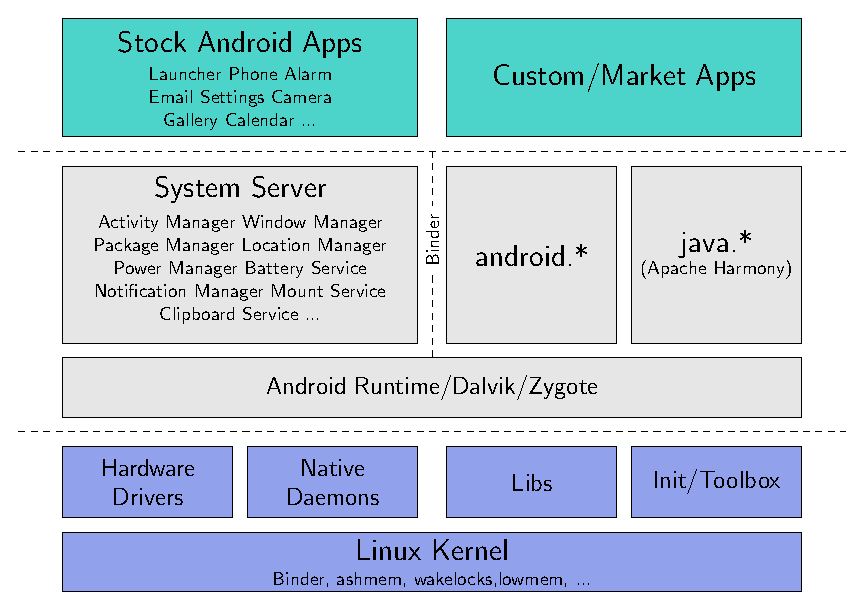
\epsfig{file=Stack.eps, width=3in,}
\caption{The Android application stack~\cite{systemserver}}
\label{fig:android}
\end{figure}

Android has one main application called the system process. The system process contains services responsible for performing the main
tasks of the system, including:
\vspace{-10pt}
\begin{description}
 \item [ActivityManager] manages the life-cycle and interaction of all the activities running on the system
 \item [WindowManager] allows applications to draw on the screen and forwards UI input to the application.
 \item [PackageManager] stores information on the application packages installed on the device
\end{description}
\vspace{-5pt}
All Android applications follow a single-threaded design in which the main thread of the application handles all application
events~\cite{AndroidDocs}. This structure is commonly used by many UI frameworks since it becomes too complex to make all UI classes thread
safe~\cite{SingleThread}. In Android, this main thread is called the \texttt{Looper} thread. The \texttt{Looper} has a message queue
attached to it containing all application events to be dispatched. UI and system events are scheduled on the main \texttt{Looper} by adding
them to the message queue. The \texttt{Looper} is responsible for continuously looping through these messages and handling them
appropriately. This could include updating a widget, loading a new activity or processing an \texttt{Intent} (see below).

The main entry-point of each Android application is in its \texttt{ActivityThread} class. The \texttt{ActivityThread} class is part of the
Android framework and starts the application's \texttt{Looper} thread. It also keeps track of the application's components and handles user
and system events. Android applications also consists of the following application components:
\vspace{-10pt}
\begin{description}
\item [Activity] responsible for representing and managing an user interface. An application can consist of many
Activities.
\item [Service] performs background operations such as the pulling of messages from a server every 5 minutes. Services do not have user
interfaces and an application can have zero or more services running simultaneously.
\item [Broadcast receiver] listens for and responds to system-wide events such as network failing, low battery or screen orientation
change events.
\item [Content provider] manages application data stored on the file system, in databases, on the web or other storage medium and provides a
gateway to this data from other applications.
\end{description}
\vspace{-5pt}
These components interact with each other and with other applications using a structure called an \texttt{Intent}. An \texttt{Intent} is a
high level implementation of the Binder IPC. \texttt{Intents} are used to start Activities and Services or to provide a notification of
certain events. They are similar to messages containing a description of an operation to be performed or, often in the case of broadcasts, a
description of something that has happened and is being announced~\cite{AndroidDocs}.

\subsection{Scope of JPF-ANDROID}
The objective of JPF-ANDROID is to verify Android applications by running the application code on the JVM using a collection of different
event sequences and then to detect when certain errors occur using JPF.
%what scope of android will be modeled

The Android framework is very large and one of the main challenges of JPF-ANDROID is to decide which parts of the system to model. The more
of the Android framework is modelled, the more realistic the model is and the more errors can be found. However, if too much
of the framework is modelled the scheduling possibilities increase exponentially which means that the search space can become too big to
verify.

JPF-ANDROID focuses on verifying a single application with multiple application components and their interaction. The system service of
the Android OS is not part of the application process and runs in its own thread. To reduce scheduling possibilities, the entire system
service is not modelled but its necessary components are implemented as part of the application process. The following parts of the Android
framework is modelled:
\vspace{-10pt}
\begin{description}
 \item [ActivityManager]  manages the life-cycle of Activities and other application components.
 \item [ActivityThread]   the main entry-point to the application. It controls and manages the application components and their input.
 \item [Application components] including Activity, Service, Broadcast Receiver and Content Provider. 
 \item [Window and View structure] The view hierarchy is modelled including the widgets and the window classes.
 \item [Message queue] modelled to support script input.
\end{description}
\vspace{-5pt}
Lastly, as the application will not be communicating with outside processes, the \texttt{Intent} objects are modelled to exclude the
Binder IPC service.

\section{Development}
\subsection{JPF-ANDROID architecture}
% \begin{figure}
% \centering
% 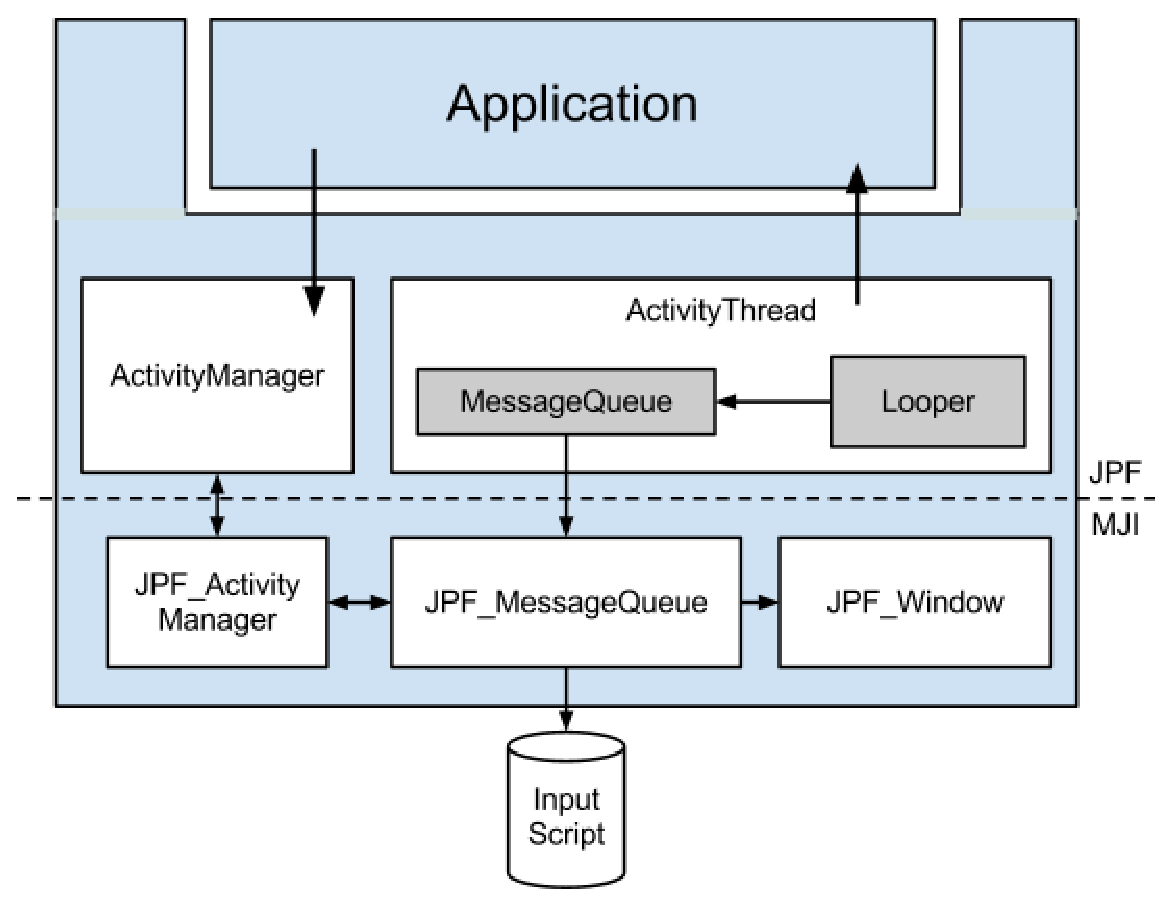
\epsfig{file=arch.eps, width=3.5in,}
% \caption{JPF-ANDROID architecture}
% \label{fig:arch}
% \end{figure}
%JPF-ANDROID BASED ON JPF_AWT  why and how does it work?
As discussed above, both Android and AWT applications have a single-threaded application design and therefore JPF-ANDROID is based on JPF-AWT's architecture.
\linebreak JPF-ANDROID models Android's message queue by using JPF's MJI
environment. When the \texttt{Looper} thread requests a new message from the message queue and it is empty, a call to the native
\texttt{JPF\_MessageQueue} class requests the next event from the scripting environment. The \texttt{JPF\_MessageQueue} class classifies
events as either UI or system events. UI events are directed to and handled by the native \texttt{JPF\_Window} class and system events by
the native \texttt{JPF\_ActivityManager} class.

% Explain what UI events are and how they are handled by android vs how they ae handled by the system
UI events include events fired by widgets such as clicking a button or selecting an item in a list view. An
Activity's UI is represented by a window object containing a view hierarchy. When the window is inflated, an object map is created in the
native \texttt{JPF\_Window} class. This map binds the name of each widget to the reference of the inflated widget object. When an UI event
is received by the native \texttt{JPF\_Window} class, the name of the target widget is looked-up in the object map and the action is then
called directly on the inflated widget object by pushing a direct call frame on the JPF call stack. 

% Explain what system events are how they are handled by android how they are handled by the system
System events use \texttt{Intent} objects to describe a event that occurred. They include events to start an Activity or Service or a
battery low notification. In the Android OS, system events are sent to the Activity manager which is modelled in JPF-ANDROID by the native
\texttt{JPF\_ActivityManager} class. This class keeps a map of Intents as they are defined in the script file. When a system event is
received, the corresponding \texttt{Intent} is looked up in the map. The \texttt{Intent} is then resolved to the relevant
component and scheduled in the application's message queue.

\subsection{The scripting environment}
% what is input script, how does it work(its function) and how are does it look
JPF-AWT's script consist of a list of UI events. These events are read one-by-one when the message queue it empty. To allow users to
script system events, variables were added to the scripting language in JPF-ANDROID. Variable names are identified by the ``@'' in front of
the variable's name as '\$' is already used in JPF-AWT to identify UI components. These variable can be used to construct most Intent
objects. For example, a script file that sends an \texttt{Intent} to start the \texttt{SampleActivity} is shown in Figure \ref{fig:start}
\begin{figure}
\frame{
\parbox{0.48\textwidth}{
{\small
{\sf 
\vspace*{2mm}
\hspace*{2mm}1. @intent1.setComponent(``SampleActivity'')\\
\hspace*{2mm}2. startActivity(@intent1)\\
\hspace*{2mm}3. \$button1.onClick()
\vspace*{2mm}
}}}}
\vspace{-18pt}
\caption{Starting SampleActivity}
\label{fig:start}
\end{figure}

JPF-ANDROID scripts also adopted the \textbf{REPEAT} and \textbf{ANY} constructs from JPF-AWT. \textbf{REPEAT} constructs repeat a list of
events a specified number of times. \textbf{ANY} constructs take a list of non-deterministic events as parameters and then uses a ChoiceGenerator and JPF's
state matching and backtracking features to visit each of the execution branches. JPF stores the state of the system before it advances
to a new state. JPF-AWT uses a JPF search listener to store and retrieve the current position of the input script in a specific state so
that the script's state is also saved.

%how and why was this scripting environment adapted
Android applications contain multiple windows - one for each Activity. This complicates the script input as each window has its own unique
set of view components, hence, a unique input sequence. Furthermore, the application flow can switch between these Activities
at any point of execution. In other words, if we do not know which Activity has the focus (or is in it's resumed state), we cannot script
the following events.

% \begin{figure}
% \centering
% 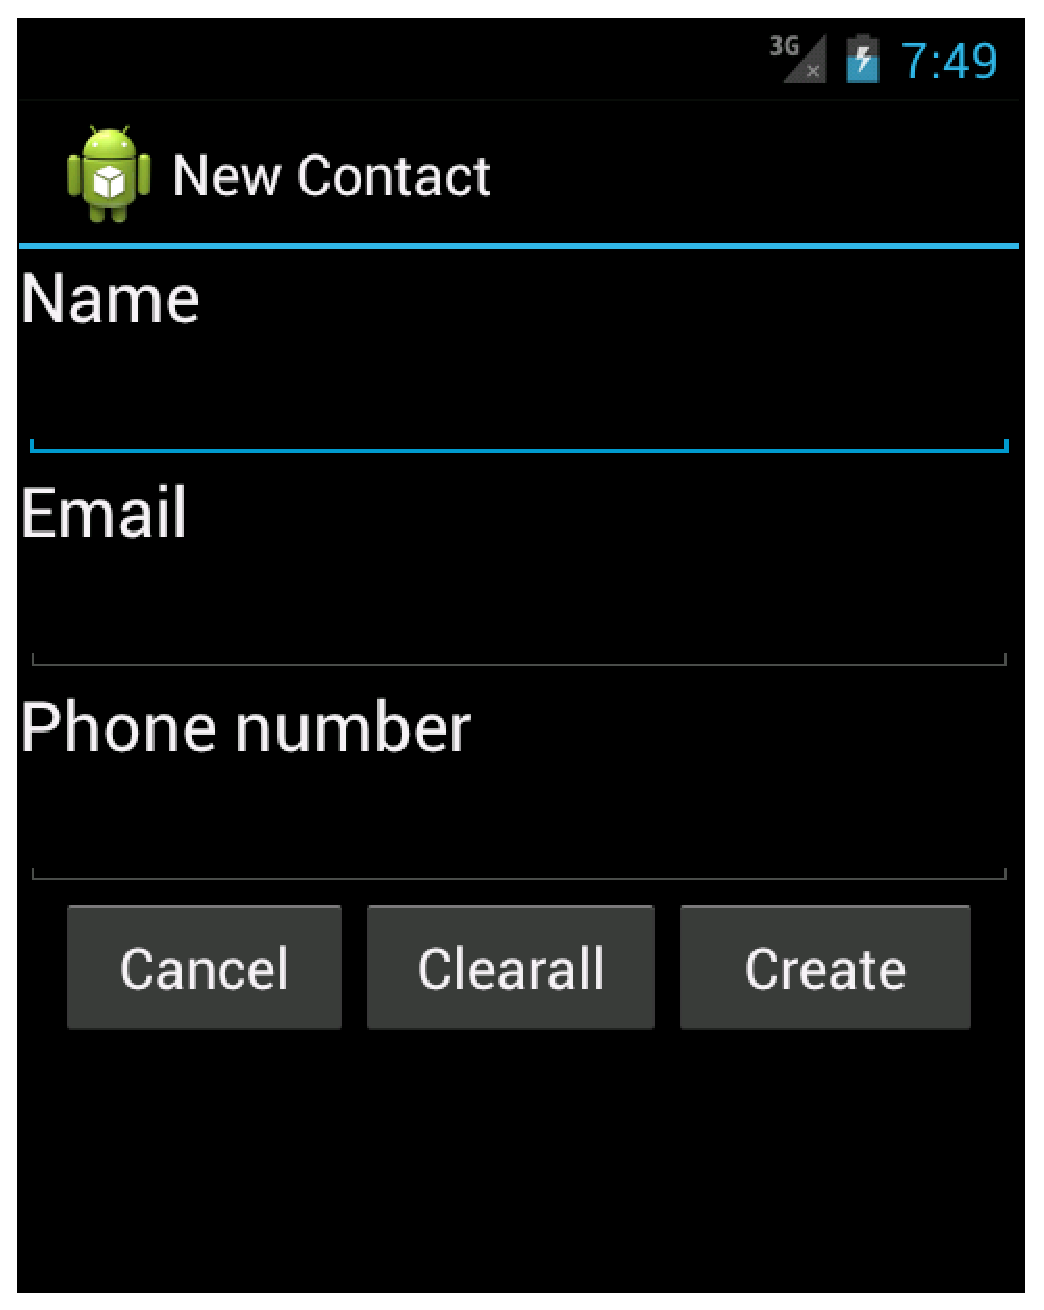
\epsfig{file=newContact.eps, width=1in,}\\
% \caption{Contacts application window}
% \end{figure}
% \begin{figure}
% {\small
% {\sf
% ...\\
% \textbf{ANY} \{ \$cancelButton.onclick(), \$clearButton.onClick()  \}
% \$nameEdit.setText(``Mary'')\\
% \$createButton.onClick()\\
% ...
% }
% }
% \caption{Input script for ``New Contact'' window}
% \end{figure}
Let us take a Contacts Android application as an example. The application has two Activities: the \texttt{ListContactsActivity} and the
\texttt{NewContactActivity}. The \texttt{ListContactsActivity} contains a list of the stored contacts and a button to add a new contact that directs the
user to the \texttt{NewContactActivity}. The \texttt{NewContactActivity} contains two buttons: the clear button stays on the current Activity and clears its
fields and the create button starts the \texttt{ListContactsActivity}. Now let us look at Figure \ref{fig:contact} containing the input
sequence for the \texttt{NewContactActivity}.

\begin{figure}
\frame{
\parbox{0.48\textwidth}{
{\small
{\sf 
\vspace*{2mm}
\hspace*{2mm}1. @startIntent.setComponent(``ListContactsActivity'')\\
\hspace*{2mm}2. startActivity(@startIntent)\\
\hspace*{2mm}3. \$createContactButton.onClick()\\
\hspace*{2mm}4. \$nameEdit.setText(``Mary'')\\
\hspace*{2mm}5. \textbf{ANY} \{ \$<create\,|\,clear>Button.onClick()\}\\
\hspace*{2mm}6. \$nameEdit.setText(``Maria'')\\
}}}}
\vspace{-15pt}
\caption{Original script for Contacts application}
\label{fig:contact}
\end{figure}

The problem occurs in the ANY structure. When the create button is clicked the application changes to the ListContactsActivity
and the following event is not valid any more. This drastically restricts the number of sequences that can be scripted in the file. To
address this issue, we included the use of sections in the input script (see Figure \ref{fig:contact2}). Each section groups the input
events of a specific Activity. Now, if the create button is pressed, the \texttt{ListContactsActivity} will be started and the events
specified in its section will start executing again.

\begin{figure}
\frame{
\parbox{0.48\textwidth}{
{\small
{\sf 
\vspace*{2mm}
\hspace*{2mm}1.\; \textbf{SECTION} default \{\\
\hspace*{2mm}2.\; \hspace*{5mm}@startIntent.setComponent(``ListContactsActivity'')\\
\hspace*{2mm}3.\; \hspace*{5mm}startActivity(@startIntent)\\
\hspace*{2mm}4.\; \}\\
\hspace*{2mm}5.\; \\
\hspace*{2mm}6.\; \textbf{SECTION} ListContactsActivity \{\\
\hspace*{2mm}7.\; \hspace*{5mm}\$createButton.onClick()\\
\hspace*{2mm}8.\; \hspace*{5mm}\$list.setSelectedIndex([0-3])\\
\hspace*{2mm}9.\; \}\\
\hspace*{2mm}10. \\
\hspace*{2mm}11. \textbf{SECTION} NewContactActivity \{\\
\hspace*{2mm}12. \hspace*{5mm}\$nameEdit.setText(``Mary'')\\
\hspace*{2mm}13. \hspace*{5mm}\textbf{ANY} \{ \$<create\,|\,clear>Button.onClick()\}\\
\hspace*{2mm}14. \hspace*{5mm}\$nameEdit.setText(``Maria'')\\
\hspace*{2mm}15. \}
\vspace*{2mm}
}}}}
\vspace{-15pt}
\caption{Adding sections to the input script}
\label{fig:contact2}
\vspace{-10pt}
\end{figure}

The addition of the sections in the input script lead to infinite event sequences. In the above example, an infinite loop occurs when the
create button is pressed on the \texttt{NewContactActivity} window. This will stop the execution of the \texttt{NewContactActivity} section and restart
the \texttt{ListContactsActivity} section's events. When the \texttt{ListContactsActivity}'s section is restarted, it again clicks on the create button
restarting the \texttt{NewContactActivity}. To address this issue, JPF-ANDROID keeps record of its current Activity. The scripting environment was
also adapted to store the current position in each visited Activity's script section. If a branch returns to a previously visited
Activity, its current position in its section is looked up and instead of restarting the section, it continues from its previous position.

\subsection{Case studies}
%calculator
%how does application look and work
The first application is a scientific calculator. The calculator has two Activities: a simple view that
displays basic arithmetic operations and a scientific view that displays more complex arithmetic operations. When the user switches
between these Activities, the current state of the calculator is preserved. This state includes the intermediate values and current
operation. This state information is bundled with the \texttt{Intent} that starts the next Activity.

\begin{figure}
\frame{
\parbox{0.48\textwidth}{
{\small
{\sf 
\vspace*{2mm}
\hspace*{2mm}1. \textbf{SECTION} SimpleActivity  \{\\
\hspace*{2mm}2. \hspace*{5mm}\textbf{ANY} \{\,\$button[0-9].onClick()\,\}\\
\hspace*{2mm}3. \hspace*{5mm}\textbf{ANY} \{\,\$button<Plus|Minus|Mul|Div|More>.onClick()\,\}\\
\hspace*{2mm}4. \hspace*{5mm}\textbf{ANY} \{\,\$button[0-9].onClick()\,\}\\
\hspace*{2mm}5. \hspace*{5mm}\$buttonEquals.onClick()\\
\hspace*{2mm}6. \}\\
\hspace*{2mm}7. \textbf{SECTION} ScientificActivity  \{\\
\hspace*{2mm}8. \hspace*{5mm}\textbf{ANY} \{\,\$button<Sin|Cos|Tan>.onClick()\,\}\\
\hspace*{2mm}9. \}\\
}}}}
\vspace{-15pt}
\caption{Input script for Calculator application}
\label{fig:calc}
\vspace{-10pt}
\end{figure}


%what errors can occur
The calculator application contains two errors. When the user divides a value by zero, an uncaught
\texttt{ArithmeticException} is thrown by the application which causes Android to kill the application. Secondly, the application neglected
to attach the state information to the \texttt{Intent} that is passed to the next Activity. When the user switches to the other Activity a
\texttt{NullPointerException} is thrown when it tries to read the state information from the \texttt{Intent}. 

To detect these errors we will use the test script in Figure~\ref{fig:calc}. The scripting environment interprets the script into the
following input sequences:
\begin{align*}
\text{<sequence>} &= \text{<simple\_seq>}\,|\,\text{<complex\_seq>}\\
\text{<simple\_seq>} &= \text{number},\,\text{simple\_op},\,\text{number},\,\text{equals}\\
\text{<complex\_seq>} &= \text{number},\,\text{complex\_op}\\
\text{simple\_op} &= \text{``+''}\,|\,\text{``-''}\,|\,\text{``}\times\text{''}\,|\,\text{``}\div\text{''}\\
\text{complex\_op} &= \text{``sin''}\,|\,\text{``cos''}\,|\,\text{``tan''}\\
\text{equals} &= \text{``=''} \\
\text{number} &= \text{``0''\,|\,``1''\,|\,``2''\,|\,``3''\,|\,``4''\,|\,``5''\,|\,``6''\,|\,``7''\,|\,``8''\,|\,``9''}
\end{align*}
Each of the ten number buttons are pressed followed by a simple operation and another number or a complex operation. Although it is possible
to input numbers consisting of multiple digits including floating point numbers, for illustration purposes this was left out of the input script.
JPF is automatically configured to detect thrown exceptions and to stop execution. When JPF-ANDROID was run on the application it firstly
detected the \texttt{ArithmenticException} due to the division by zero:

\vspace*{-10pt}
\begingroup
 \fontsize{6pt}{7pt}\selectfont
\begin{verbatim}
====================================================== results
error #1: gov.nasa.jpf.jvm.NoUncaughtExceptionsProperty 
         "java.lang.ArithmeticException: Division by zero  at ..."
====================================================== statistics
elapsed time:       00:00:01
states:             new=76, visited=0, backtracked=63, end=30
search:             maxDepth=13, constraints hit=0
choice generators:  thread=7 (signal=0, lock=3, shared ref=0), data=39
heap:               new=3455, released=2105, max live=1507, gc-cycles=74
instructions:       76796
max memory:         117MB
loaded code:        classes=145, methods=2064
======================================================
\end{verbatim}
\endgroup
\vspace*{-10pt}
After this error was fixed JPF-ANDROID detected the \texttt{NullPointerException} in the same way.

Both of these errors would have been difficult to detect with unit testing. The \texttt{ArithmenticException} is challenging due
to the many possible input sequence combinations. If a test case did not specifically identify this as a point of interest, unit testing
would not have detected this error. The second error is challenging to detect due to the fact that it only occurs when the flow of Activity
classes are tested.

% deadlock
%how does application look and work
The next case study is a very simple application demonstrating how JPF-ANDROID detects a deadlock in a Android application. When the
\texttt{Looper} thread of an application is caught in a deadlock, the Android OS kills the application and displays an
Application Not Responding (ANR) dialog. However, Android does not detect a deadlock if it occurs between other asynchronous threads. This
sample application spawns two asynchronous threads that deadlock. The application has one Activity with two
buttons. The first button spawns the first thread and the second button spawns the second thread. After a while these two thread deadlock
and are then blocked forever, waiting for each other. The input script for the application is given in Figure \ref{fig:deadlock}. JPF is then
configured to listen for deadlocks and schedules the threads in all possible ways to detect the deadlock.

\begin{figure}

\frame{
\parbox{0.48\textwidth}{
{\small
{\sf 
\vspace*{2mm}
\hspace*{2mm}1. \textbf{SECTION} DeadlockActivity  \{\\
\hspace*{2mm}2. \hspace*{5mm}\$button1.onClick()\\
\hspace*{2mm}3. \hspace*{5mm}\$button2.onClick()\\
\hspace*{2mm}4. \}\\
}}}}

\caption{Input script for Deadlock application}
\label{fig:deadlock}
\vspace{-10pt}
\end{figure}

\vspace*{-10pt}
\begingroup
 \fontsize{6pt}{7pt}\selectfont
\begin{verbatim}
 ====================================================== thread ops #1
   1       1     trans          loc            : stmt
------- ------- ---------------------------------------------------
B:1003     |      54  DeadlockActivity.java:82 : bower.bowBack(this);
   |    B:1000    54  DeadlockActivity.java:82 : bower.bowBack(this);
L:1000     |      54  DeadlockActivity.java:56 : friend[0].bow(friend[1]);
   |    L:1003    18  DeadlockActivity.java:56 : friend[0].bow(friend[1]);
   S       |       6
   |       S       3
====================================================== results
error #1: gov.nasa.jpf.jvm.NotDeadlockedProperty 
         "deadlock encountered:   thread java.lang.Thread:{i..."
====================================================== statistics
elapsed time:       00:00:01
states:             new=55, visited=13, backtracked=67, end=1
search:             maxDepth=10, constraints hit=0
choice generators:  thread=26 (signal=0, lock=11, shared ref=0), data=7
heap:               new=1430, released=375, max live=1040, gc-cycles=67
instructions:       12661
max memory:         117MB
loaded code:        classes=140, methods=1792
======================================================
\end{verbatim}
\endgroup
\vspace*{-10pt}
\section{Future Work}
Currently JPF-ANDROID can detect deadlocks, race conditions and other property violations in Android applications. The next challenge is
modelling the extra Android libraries. This is because most Android applications make use of many Android specific
libraries such as the sqlite database connector, HTTP connections or the media player libraries.

Another extension that will be added to JPF-ANDROID is coverage testing. JPF has many coverage extensions available so we will be adapting
one these extensions to work on Android applications~\cite{coverage}. Coverage testing is especially important to find errors related to the Android Activity
life cycle such as the null pointer exception mentioned above.

\section{Conclusion}
The paper discussed the design and implementation of JPF-ANDROID. JPF-ANDROID is still under development and currently only models
the core libraries needed to verify a basic Android application. It allows Android applications to be tested using JPF's proven verification
techniques and can successfully detect common Java errors such as runtime exceptions and deadlocks.

This extension provides a basis on which Android applications can be tested. It can later be extended to verify functional requirements and identify Android specific errors using JPF's listener mechanism.

% \vspace*{5pt}
% The following two commands are all you need in the
% initial runs of your .tex file to
% produce the bibliography for the citations in your paper.
\bibliographystyle{abbrv}
\scriptsize
\bibliography{paper}  % sigproc.bib is the name of the Bibliography in this case

\end{document}
